\section{Использование Backbone.JS}
Первоначально было решено использовать для реализации данный инструмент. Основными предпосылками были легковесность (около 6 Кб), высокая интеграция с jQuery и высокий контроль процесса написания приложения. При написании данного приложения была задействована структура каталогов, отображенная на рисунке \ref{backbone_structure}. В директории css находятся таблицы стилей, в js находится код моделей, контроллеров и роутеров. В файле index.html  В каталоге libs находятся различные библиотеки, задействованные при написании данного приложения.

\begin{figure}[h]
\center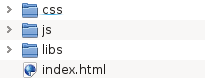
\includegraphics[width=0.4\textwidth]{backbone_structure}
\caption{Структура каталогов}\label{backbone_structure}
\end{figure}

\subsection{Реализация представлений}

Первым делом были написаны шаблоны представлений:

\begin{enumerate}
 \item Представление для создания нового задания. .
 \item Представление для просмотра списка поставленных задач.
 \item Представление для вывода подробной информации об исследовании.
 \item Шаблон для построения графика результата.
\end{enumerate}

Представление для создания нового задания получается довольно динамическим: форма генерируется налету, ее компоненты зависят от выбранного алгоритма, что приводит к перестройке формы при смене алгоритма. В более-менее сложных разметках использование HTML кода внутри JavaScript довольно бессмысленная затея. Код становится запутанным и сложнее для понимания, а также теряются преимущества использования среды разработки. К сожалению, библиотека Backbone.JS не имеет встроенного шаблонизатора --- авторы оставляют выбор за разработчиком. Поэтому был написан свой, основанный на шаблонизаторе Mustache из библиотеки Underscore.js. Его основное отличие в том, что заимствованная библиотека позволяет хранить шаблон только в виде строки, в то время как написанный шаблонизатор из файлов. Шаблон представляет собой скрипт с типом \textbf{text/template} и имеет уникальный идентификатор. Тело шаблона представлено в виде расширенного HTML и компилируется написанной функцией template. В ходе компиляции происходит санитизация полученных данных, интерполяция переменных и необходимые вычисления для чего используется специальный синтаксис <\% ... \%> и <\%= … \%>. Пример кода шаблона отображен на рисунке \ref{template_example}. Скомпилированный шаблон отражен на рисунке \ref{new_issue}.

\begin{figure}[ht]
\center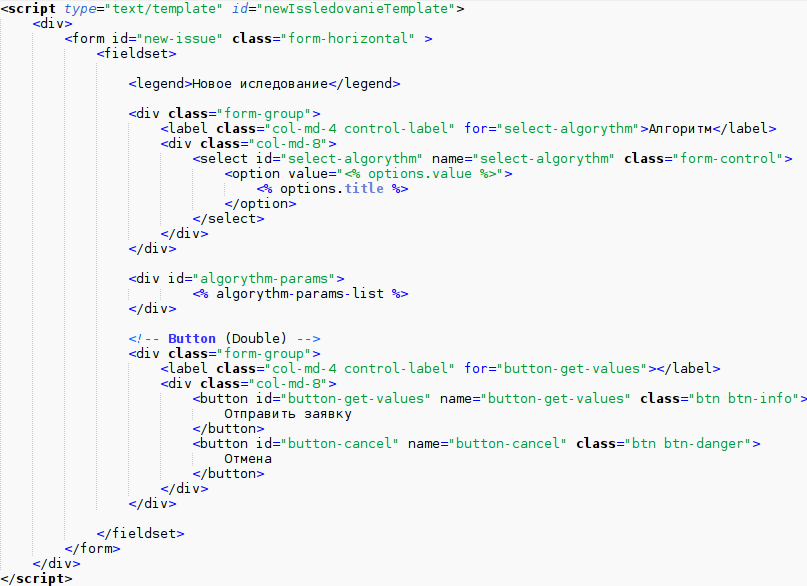
\includegraphics[width=\textwidth]{template_example}
\caption{Пример шаблона}\label{template_example}
\end{figure}

\begin{figure}[ht]
\center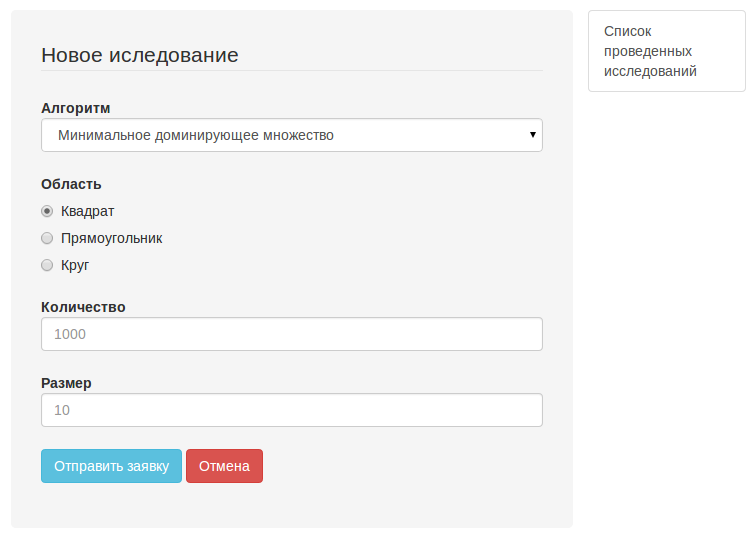
\includegraphics[width=\textwidth]{new_issue}
\caption{Пример шаблона}\label{new_issue}
\end{figure}

Для быстрой разработки и верстки шаблонов в ходе создании представлений активно использовалась библиотека Twitter Bootstrap. Это свободный набор инструментов, включающий в себя CSS шаблоны оформления веб-форм, кнопок, меток, блоков навигации. Он использует самые современные наработки в области CSS и HTML и позволяет сэкономить время и усилия, используя шаблоны дизайна. Также все компоненты платформы Bootstrap используют единый стиль благодаря чему веб-страницы имеют приятный интерфейс.

Представление для просмотра списка поставленных задач не отличается ни чем примечательным: это нумерованный список результатов. Результат отображен на рисунке \ref{list}. Результаты, находящиеся в очереди, обведены серым фоном и недоступны для подробного просмотра. Вывод подробной информации об исследовании аналогичен созданию нового. Если результатом исследования является график, то задействуется специальный шаблон. Он позволяет курсором подробно изучать полученные значения характеристик в различных точках графика. Скомпилированный шаблон отражен на рисунке \ref{result}.

\begin{figure}[ht]
\center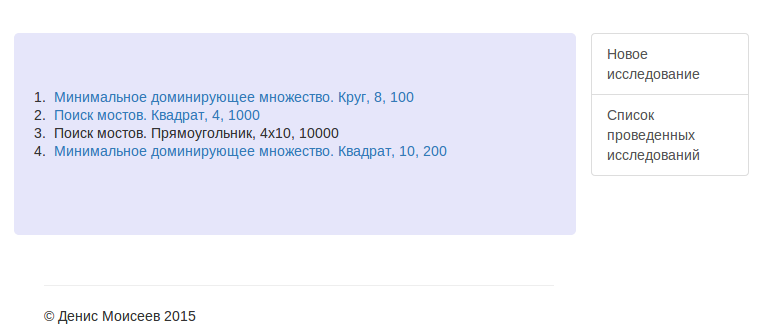
\includegraphics[width=\textwidth]{list}
\caption{Пример шаблона}\label{list}
\end{figure}

\begin{figure}[ht]
\center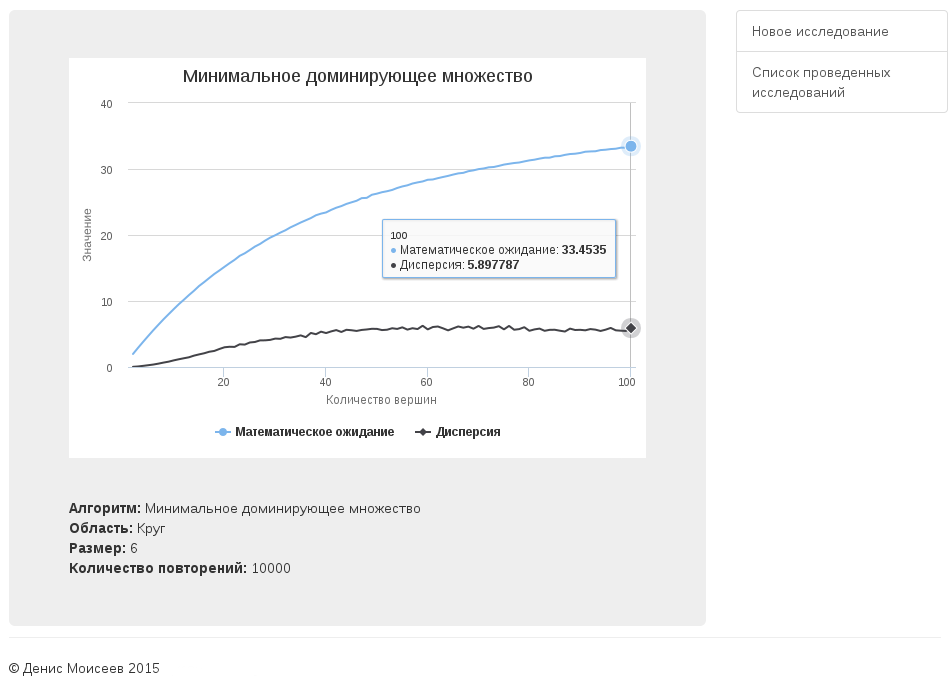
\includegraphics[width=\textwidth]{result}
\caption{Пример шаблона}\label{result}
\end{figure}

\lstset{ %
  language=JavaScript
}

После того как были подготовлены основные шаблоны, можно приступить к созданию вида в Backbone. Для этого достаточно расширить базовый класс, задать базовый тег и переопределить метод render():
\begin{lstlisting}
var IssueListView = Backbone.View.extend({
  tagName: 'ol',
  template: template('listTemplate'),
  render: function() {
    var elem = this.template(this.toJSON());
    this.$el.html(elem);
  }
});
\end{lstlisting}
Исходные коды всех представлений и шаблонов отображены в приложении А.

\subsection{Хранение данных}

Представления созданы, теперь необходимо позаботиться о хранении данных в процессе работы программы. Данные в программах, написанных с использованием Backbone.js хранятся в моделях --- специальных конструкторов объектов с уже готовым набором служебных методов. Создание модели происходит достаточно просто --- необходимо расширить базовую модель:
\begin{lstlisting}
var IssueModel = Backbone.Model.extend({
  defaults: {
    type: null,
    area: null,
    size: 0,
    step_count: 0,
    vertex_count: 0
  }
});
\end{lstlisting}
Таким образом, создается новый класс Model, который принимает параметром анонимный объект и класс модели наполняется значениями. После создания класса модели, для инстанцирования экземпляра класса можно воспользоваться стандартным способом при помощи new, при этом конструктору передается объект с данными, которые попадут в экземпляр класса:
\begin{lstlisting}
var issue = new IssueModel({
  type: "min_dom",
  area: "circle",
  size: 8,
  step_count: 1000,
  vertex_count: 100
});
\end{lstlisting}
Для доступа к атрибутам модели или создания новых в процессе исполнения программы необходимо воспользоваться методами get() и set(). В отличие от прямого доступа к данным, использование getter'ов и setter'ов инкапсулирует доступ к данным экземпляра, а также позволяет контроллерам отреагировать на изменение модели --- произойдет рассылка события 'change' всем подписанным контроллерам на этот экземпляр.

Для описания модели исследования была спроектирована следующая структура модели, отображенная на рисунке \ref{issue_model_backbone}. Самые основные атрибуты, которые присутствуют у большинства исследований (алгоритм, тип исследуемой области, размер области, количество вершин, количество повторений запуска алгоритма и основные статистические характеристики) были вынесены в класс модели. Остальные атрибуты, которые присутствуют только у конкретных алгоритмов могут быть легко добавлены в модель при помощи метода set().

\begin{figure}[ht]
\center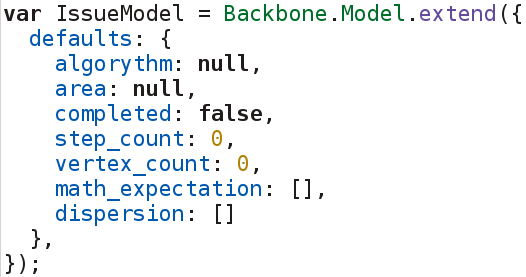
\includegraphics[width=0.75\textwidth]{issue_model_backbone}
\caption{Реализация модели исследования}\label{issue_model_backbone}
\end{figure}

Пока что создана только модель описания исследования. Но в приложении необходимо оперировать не одним объектом. Конечно, можно создать нужное количество экземпляров модели, потом для каждой создать отдельные экземпляры представлений и связать их. Однако, в таком случае код будет захламлен целой кучей экземпляров моделей и представлений. В таком случае, для хранения списка результатов существует удобное решение, встроенное в Backbone --- коллекции.

Коллекции в Backbone.js по сути являются массивами экземпляров моделей. Однако, помимо этого у них есть дополнительный функционал, который делают их вне конкуренции по сравнению с обычными массивами.

Коллекции создаются путем расширения базовой коллекции. Чтобы связать коллекцию с моделью, при ее создании в свойстве model передают ссылку на модель. Например:
\begin{lstlisting}
var IssueCollection = Backbone.Collection.extend({
  model: IssueModel
});
\end{lstlisting}
После этого можно создавать экземпляр коллекции и передавать либо ссылку на существующий экземпляр модели, либо массив с несколькими экземплярами моделей:
\begin{lstlisting}
var issue2 = new IssueModel({
  type: "bridge",
  area: "square",
  size: 4,
  step_count: 500,
  vertex_count: 100
});

var issueCollection = new IssueCollection([issue, issue2]);
\end{lstlisting}
После создания коллекции понадобится возможность создания и удаления моделей из коллекции. Для этого можно воспользоваться методами add() и remove(). Основное преимущество от использования коллекций заключается в том, что при изменении списка результатов произойдет автоматическое обновление представлений благодаря системе событий. Любое событие, которое сработает на модели в коллекции также сработает и напрямую --- для удобства --- на коллекции. Это позволяет напрямую слушать события изменения отдельных атрибутов любой модели в коллекции \cite{backbone}.

\subsection{Реализация логики приложения}

Теперь, когда готовы модель и представления пришло время соединить их контроллерами. Для начала нам необходимо отслеживать текущее состояние приложения. Необходимо определить --- создает ли пользователь новую заявку или же он просматривает список проведенных исследований. А может вообще запрашивает результат.  Конечно эту информацию можно хранить в каких-то внутренних переменных, но обычно попутно нужно решить еще одну задачу — пользователь должен иметь возможность сохранять текущее состояние приложения, чтобы потом вернуться к нему, как будто перерыва во времени и не было вовсе. Часть информации, такая как созданные заявки, их статус и подробная информация о проведении исследования, хранится на сервере, чтобы потом быть загруженной при запуске приложения, а часть, та которая отражает текущее состояние пользовательского интерфейса, обычно хранится в адресной строке браузера. 

Обычно нам необходимо отслеживать изменения в адресной строке, чтобы по-разному реагировать на них, а также иметь возможность самим менять адресную строку, в случае если состояние приложения изменилось. В Backbone есть встроенные средства для легкой реализации подобного поведения.
\begin{enumerate}
\item Роутер (Router). Занимается маршрутизацией. В этот объект записываются все возможные шаблоны (роуты) для адресной строки, а также соответствующая каждому шаблону функция, которая будет вызвана, в случае если текущая адресная строка будет ему удовлетворять\cite{backbone}.

\item История (History). Запускает отслеживание изменений. У объекта Backbone.History есть только один встроенный метод start. Backbone поддерживает отражение текущего состояния в адресной строке как с помощью хэшей (\#issue/108), так и с помощью History API (issue/108) в тех браузерах, которые это поддерживают, деградируя до использования хешей в старых браузерах\cite{backbone}.
\end{enumerate}

Роутер создается путем расширения базового класса Backbone.Router. Все маршруты записываются в виде ассоциативного массива в свойство routes. В паре ключ-значение в ключ записывается шаблон для адресной строки, а в значение --- строка с названием функции, которая будет вызвана в случае совпадения. Сами вызываемые функции записываются в свойства будущего класса роутера:
\begin{lstlisting}
AppRouter = Backbone.Router.extend({
  routes: {
    '': 'list_issues',
    "issue": 'list_issues',
    "issue/new": 'create_issue',
    'issue/:id': 'display_issue',
    '*': 'list_issues'
  },
  list_issues: function() {
    issues.fetch();
    issues_view = new IssueListView({collection: issues});
    content_element.html(issues_view.render());
  },
  display_issue: function(id) {
    issue = issues.get(id);
    content_element.html(template('IssledovaniaTemplate')(issue));
  }
\end{lstlisting}

Каждая такая функция является контроллером в модели проектирования MVC. В данной работе понадобилось написать три таких контроллера: для отображения списка результатов (отображен выше), для создания новой заявки и для отображения конкретного результата исследования. Начнем с реализации контроллера для создания новой заявки. Получим данные об алгоритмах с сервера, заполним шаблон. Также необходимо обработать отправление результата веб-сервису:
\begin{lstlisting}
create_issue: function() {
  var data = algorythms.fetch();
  content_element.html(template('newIssledovanieTemplate')({
    options: data,
    algorythm_params_list: function() {data.render()}
  }));
  $('#submit').submit( function( e ) {
    var data = $(this).serializeArray();
    var issue = new IssueModel(data);
    issue.save();
    issue.once("sync", function(issue){
      issues.add(issue);
    });
    location.href = "#";
    e.preventDefault();
  });
},
\end{lstlisting}
Данный код отображен схематически, полная реализация контроллеров доступна в приложении Б. Контроллер для отображения результата не особым не отличается и также был отображен выше.